This section presents an example how a problem could be diagnosed and
appropriate procedure applied by the operator of a WR Switch based on the
general status objects described in section \ref{sec:snmp_exports:basic}. The
screenshots included in this example were made from \emph{Diamon} tool used at
CERN for diagnostics. Any other SNMP manager (like \emph{Nagios} or
\emph{Icinga}) can be used to fetch the value of these status objects.

\begin{enumerate}
  \item Operator gets an e-mail/sms alarm or notices in the SNMP manager that
    the status of a WR switch has changed to \texttt{Error}
    (fig.\ref{fig:diamon:wrs_error})
  \item By checking the general status objects
    (\texttt{glshyperlink{WR-SWITCH-MIB::wrsOSStatus}},
    \texttt{\glshyperlink{WR-SWITCH-MIB::wrsTimingStatus}},
    \texttt{\glshyperlink{WR-SWITCH-MIB::wrsNetworkingStatus}}) one can realize
    that the problem is reported by the synchronization subsystem. The value of
    \texttt{\glshyperlink{WR-SWITCH-MIB::wrsTimingStatus}} is \emph{2}= error
    (fig.\ref{fig:diamon:wrs_sync_error}).
  \item Following the tree structure of status objects from figure
    \ref{fig:snmp_oper}, if
    \texttt{\glshyperlink{WR-SWITCH-MIB::wrsTimingStatus}} reports an error,
    then status objects: \texttt{\glshyperlink{WR-SWITCH-MIB::wrsPTPStatus}},
    \texttt{\glshyperlink{WR-SWITCH-MIB::wrsSoftPLLStatus}},\\
    \texttt{\glshyperlink{WR-SWITCH-MIB::wrsSlaveLinksStatus}},
    \texttt{\glshyperlink{WR-SWITCH-MIB::wrsPTPFramesFlowing}} should be
    checked. In this example
    \texttt{\glshyperlink{WR-SWITCH-MIB::wrsSlaveLinksStatus}} reports an error
    (fig.\ref{fig:diamon:slave_link_error}).
  \item The operator should search section \ref{sec:snmp_exports:basic} for
    procedure to follow when
    \texttt{\glshyperlink{WR-SWITCH-MIB::wrsSlaveLinksStatus}} reports an error.
  \item In this example, the WR Switch that reports a problem works in the
    Boundary Clock mode, which means that the first step according to the
    procedure should be checking a fiber connection on the slave port.
  \item Plugging the fiber to the slave port fixes the problem and WR Switch
    does not report more errors (fig.\ref{fig:diamon:wrs_ok}).
\end{enumerate}

\begin{figure}
  \begin{center}
    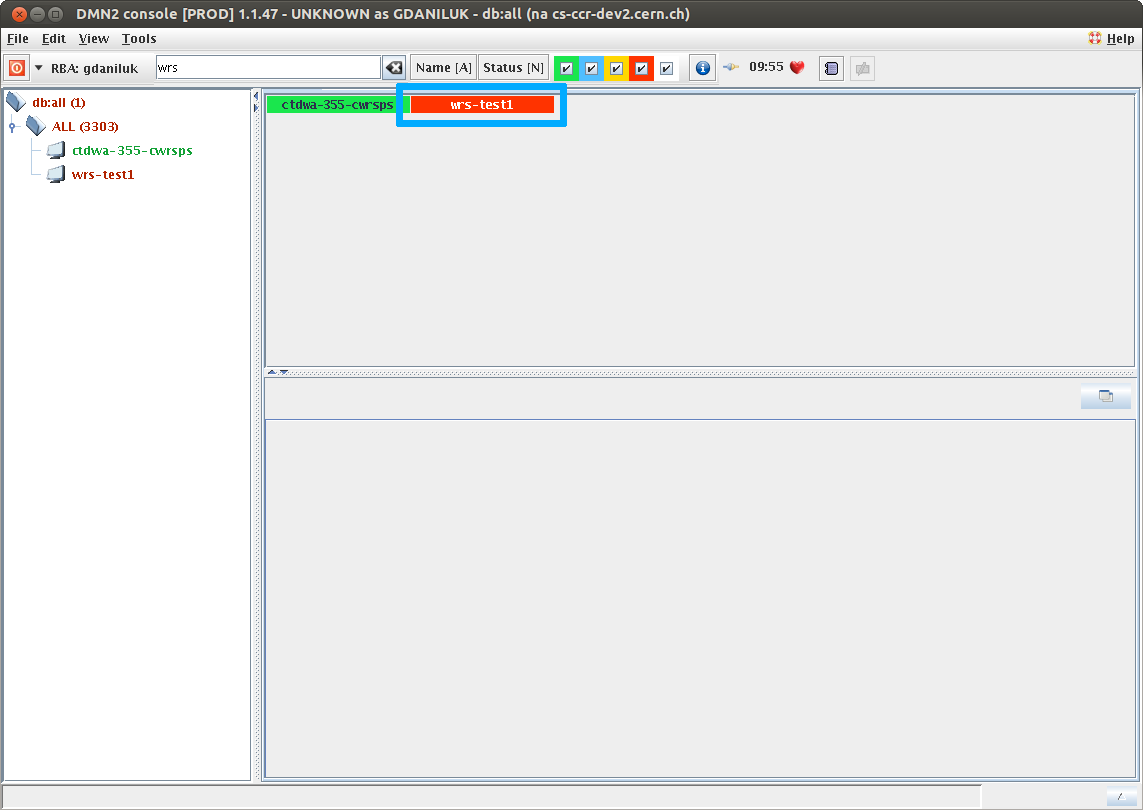
\includegraphics[width=.9\textwidth]{img/wrs_error.png}
    \caption{SNMP manager reports an error on a WR Switch}
    \label{fig:diamon:wrs_error}
  \end{center}
\end{figure}

\begin{figure}
  \begin{center}
    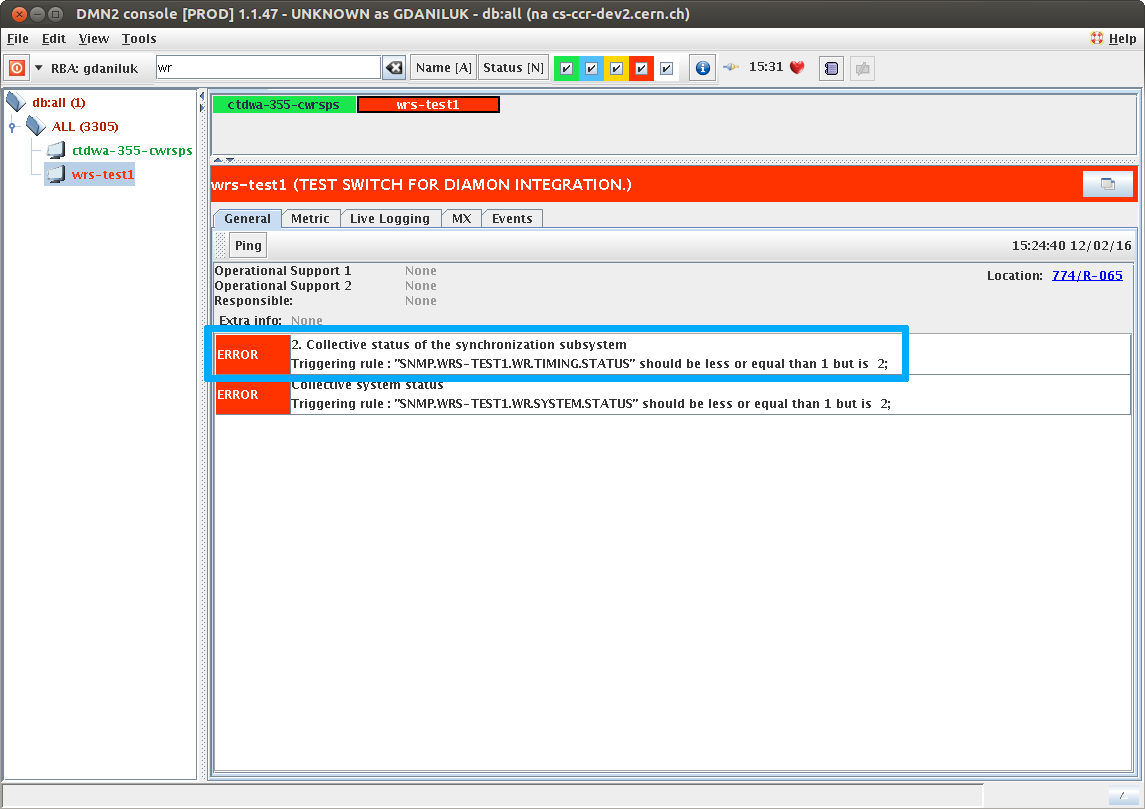
\includegraphics[width=.9\textwidth]{img/wrs_sync_error.png}
    \caption{WR Switch has problem with the synchronization subsystem}
    \label{fig:diamon:wrs_sync_error}
  \end{center}
\end{figure}

\begin{figure}
  \begin{center}
    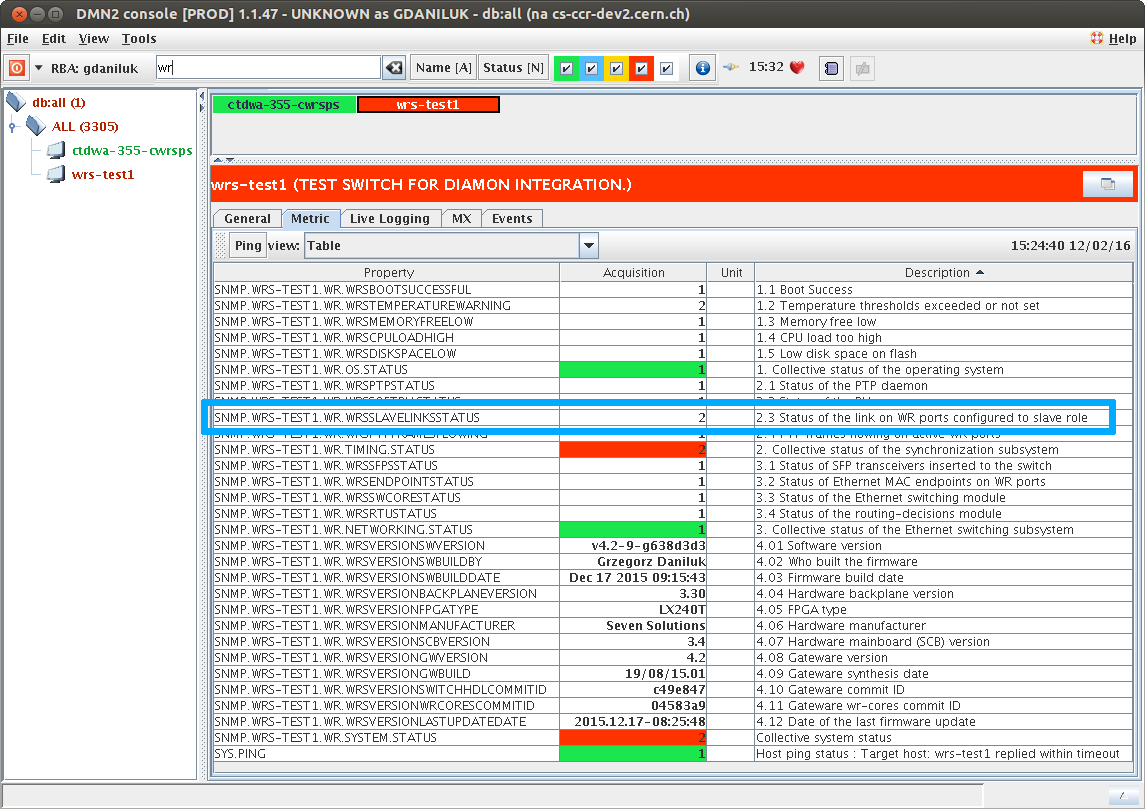
\includegraphics[width=.9\textwidth]{img/wrs_link_error.png}
    \caption{\texttt{wrsSlaveLinksStatus} object reports an error}
    \label{fig:diamon:slave_link_error}
  \end{center}
\end{figure}

\begin{figure}
  \begin{center}
    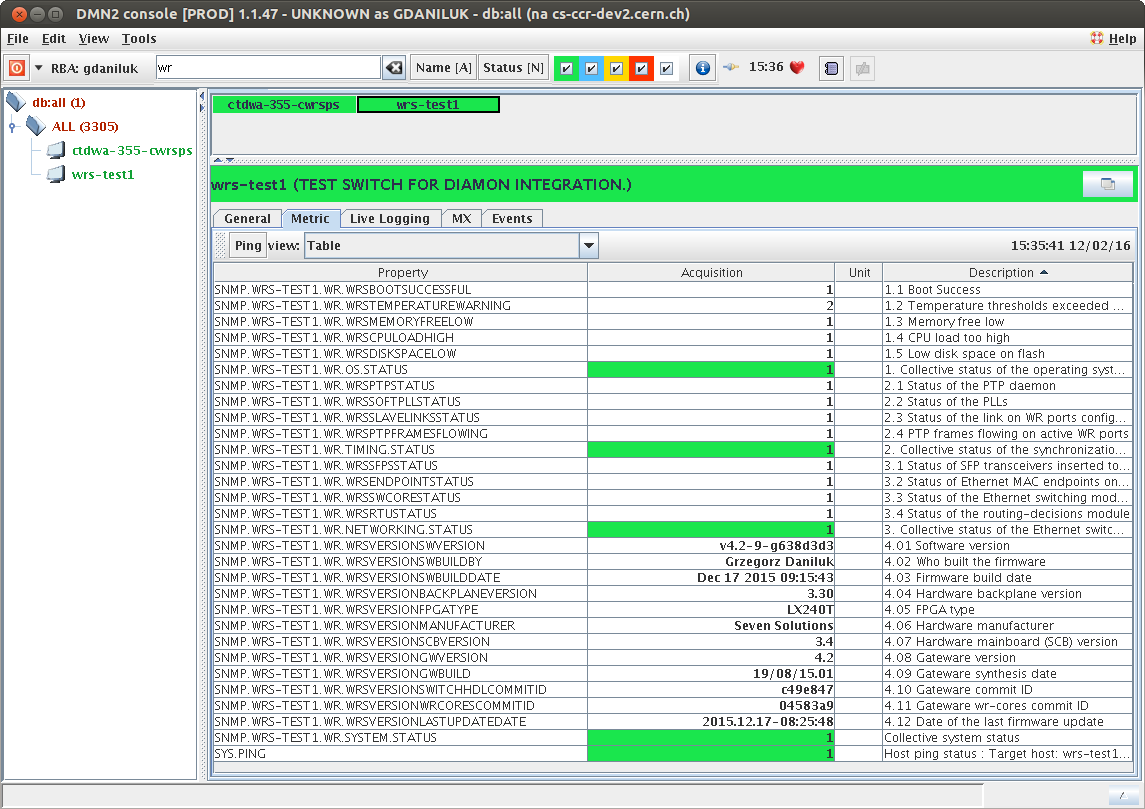
\includegraphics[width=.9\textwidth]{img/wrs_ok.png}
    \caption{WR Switch does not report any errors}
    \label{fig:diamon:wrs_ok}
  \end{center}
\end{figure}
